% Chapter 2: Lit Review
\chapter{Literature Review}
\label{chapter:lit-review}

\graphicspath{ {report/C2 Literature Review/assets/} } 

% 2.1: EEG and neuroanatomy
\section{Basic neurophysiology}

\subsection{Electrophysiology}
EEG relies on electrophysiological activity generated by electro-chemical neurotransmitters that exchange signals between neurons in the brain \cite{bci-survey-nicolas-alonso}. Roughly speaking, when a neuron is excited by afferent action potentials (rapid changes in cell membrane potentials), postsynaptic potentials (EPSPs) are generated in its apical dendrites \cite{baillet-em-brain-mapping} (neural branches). This induces a potential difference (dipole) which results in a small flow of current from the nonexcited soma membrane to the apical dendrites where the EPSPs are present. \cite{baillet-em-brain-mapping}. This process causes both intracellular current flow within the neuron, as well as extracellular current flow. These current flows are termed \textit{primary} and \textit{secondary} or \textit{return} currents respectively. Both such currents contribute to electrical potentials measured on the scalp. However, it is believed that the source of most measurable EEG potentials arises from large collections of cortical pyramidal neurons arranged in macro-assemblies with dendrites orientated perpendicularly to the local cortical surface \cite{baillet-em-brain-mapping}, \cite{teplan-eeg-measurement}. The specific spatial positioning and simultaneous activation of these large clusters of neurons is believed to generate signals that can be measured on the scalp. Specifically, \cite{baillet-em-brain-mapping} suggests that these signals most likely arise from EPSPs in these macro-assemblies and less so due to rapidly firing action potentials that travel along the axons of excited neurons.

\subsection{Functional neuroimaging}
Various techniques exist for measuring and translating brain activity into electrical signals. These techniques are typically grouped into electrophysiological and hemodynamic. Hemodynamic techniques such as functional magnetic resonance (fMRI) and near infrared (NIR) spectroscopy measure brain activity \textit{indirectly }by tracking relative concentrations of oxyhemoglobin. The blood releases glucose to \textit{active} neurons at a greater rate than inactive ones which causes an increase in oxyhemoglobin in these active areas \cite{bci-survey-nicolas-alonso}, thereby providing a measurable proxy for cerebral activity. While hemodynamic approaches offer superior spatial resolution, they typically offer far lower temporal resolution and require complex, expensive equipment. 

EEG, on the other hand, is a electrophysiological technique that relies on the direct measurement of electrical signals generated by neural cell assemblies. Owing to the fact that it offers high temporal resolution\footnote{typically in the order of tens of milliseconds}, far lower cost than most other techniques, good portability and safety, EEG has become the most widely used neuroimaging modality \cite{bci-survey-nicolas-alonso}. It is these factors that make EEG most appropriate for this project.

\section{Electroencephalography}

\subsection{Invasive vs non-invasive techniques}

The ability to reliably detect EEG signals is made challenging by the fact that neuron potentials must pass through the skull and scalp and will unavoidably be measured in conjunction with background noise and other undesirable artefacts such as electromyography (EMG) signals. Invasive methods that require surgical implantation of electronic devices are sometimes used in order to circumvent some of these challenges. Electrocorticography or intercranial EEG is an example of an invasive method; an electrode array is placed directly on the exposed surface of the brain to measure cerebral activity. 

While invasive methods offer superior signal resolution and quality, they are clearly not suitable for this project. Non-invasive BCIs do not require any surgical intervention and only involve the placement of electrodes on the scalp of the subject. Despite the aforementioned challenges of measuring signals of poorer quality, this has the advantage of convenience, cost effectiveness, safety and minimal invasiveness.

\subsection{The nature of EEG signals}
\label{subsection:nature-of-eeg-signals}
EEG signals most commonly range in amplitude from 0.5 to $100\mu$V peak-to-peak \cite{teplan-eeg-measurement} (in the case of a healthy brain). For reference, this is roughly 100 times lower than the typical amplitude of ECG signals. It is widely believed that EEG signals show varying energy in a few distinct frequency bands depending on mental state and cognitive function of a subject \cite{baillet-em-brain-mapping}, \cite{varnavas-phd}. These frequency bands are summarised below \cite{varnavas-phd}, \cite{bci-survey-nicolas-alonso}:

\begin{table}[!htb]
\centering
\begin{tabular}{@{}ll@{}}
\toprule
\textbf{Frequency band} &
  \textbf{Physiological association} \\ \midrule
\textit{delta} (0.5 - 4Hz) &
  \begin{tabular}[c]{@{}l@{}}Usually only detected in a state of deep sleep. Excessive signal energy in the delta band \\ while awake may suggest neurological disease.\end{tabular} \\
\textit{theta} (4 - 8Hz) &
  \begin{tabular}[c]{@{}l@{}}Cognitive tasks involving association, awareness and meditation. Usually low energy\\ in this band while subject is awake.\end{tabular} \\
\textit{alpha} (8 - 13Hz) &
  \begin{tabular}[c]{@{}l@{}}Typically measured in the occipital region of the brain. Primarily related to visual processing \\ but also memory processes. Induced by closing of the eyes and relaxing and attenuated when \\ eyes are open or by thinking or mental calculation.\end{tabular} \\
\textit{beta} (12 - 30Hz) &
  \begin{tabular}[c]{@{}l@{}}A variety of mental processes such as mathematical computation, planning, high \\ level processing\end{tabular} \\ \bottomrule
\end{tabular}
\caption{Summary of commonly designated EEG signal frequency bands and their broad physiological associations}
\label{tab:c2-freq-bands}
\end{table}

It is worth noting that different areas of the brain may produce signals with different energy compositions across these frequency bands. Consequently, the particular placement of electrodes in measuring localised signals of interest is an important consideration.

\subsection{Electrode choice and placement}
An EEG is signal is most commonly measured as the potential difference over time between active and reference electrodes. A third ground electrode is used to measure differential voltage between the active and reference electrodes and thus, a minimal setup requires at least 3 electrodes in total \cite{bci-survey-nicolas-alonso}. Electrodes be used in conjunction with conductive media such as conductive gel or without and would be termed wet or dry electrodes in these two cases respectively. 

Electrodes are most commonly arranged on the scalp according to the International 10-20 system standardised by the American Electroencephalographic Society. An overview of this system is presented in Figure \ref{fig:10-20-positions}.

\begin{figure}[h]
    \centering
    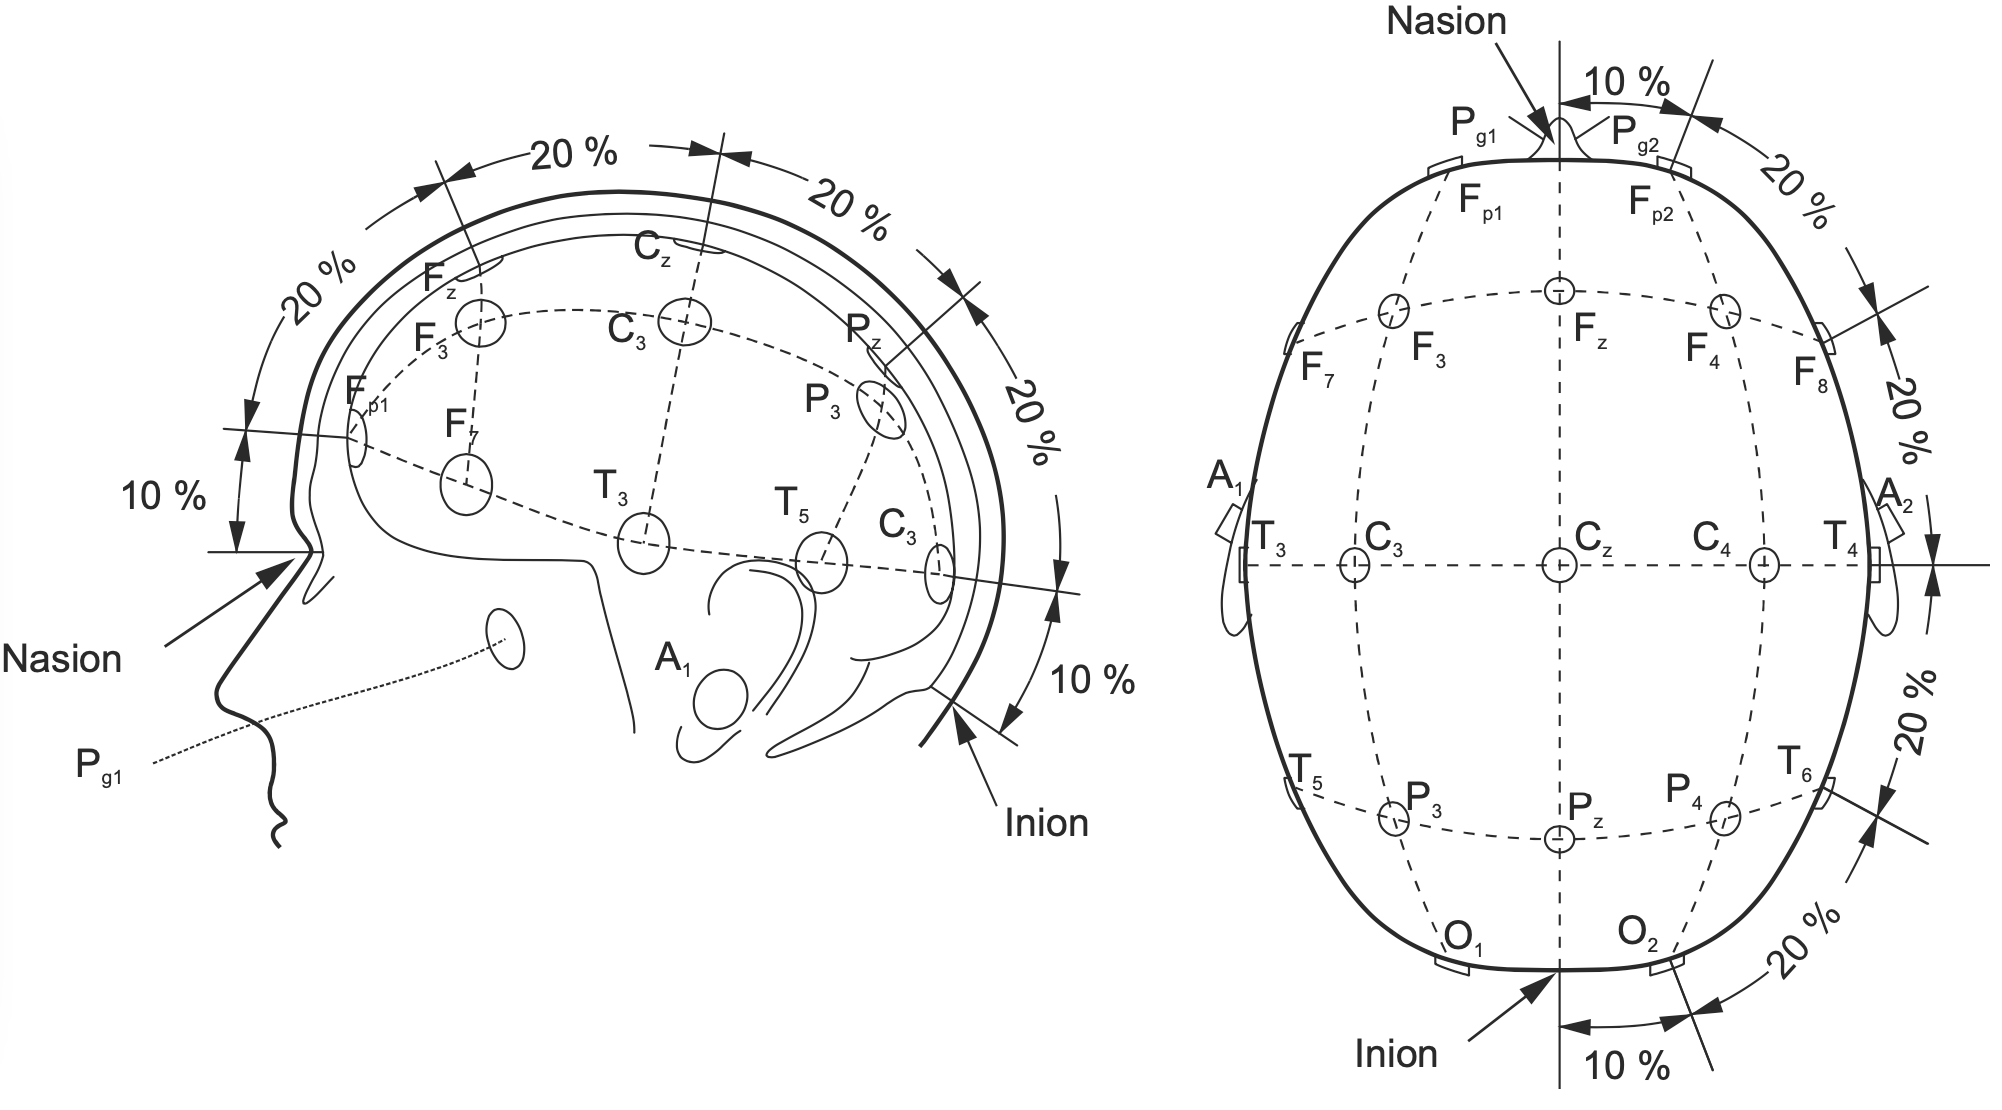
\includegraphics[width=0.8\textwidth]{10-20-electrode.png}
    \caption[Electrode positions according to the 10-20 system]{Diagram illustrating typical electrode placements using the international 10-20 system. A represents the ear lobe, C the central region, P the parietal, F the frontal and O the occipital. The \textit{naison} and \textit{inion} are used as reference locations.}
    \label{fig:10-20-positions}
\end{figure}

\subsection{BCI control signals}
The core role of a BCI is to interpret the intentions of a subject by making sense of their brain signals. These signals are comprised of a superposition of many different neuronal potentials associated with various mental tasks, most of which are not yet understood or clearly identifiable. However, there are some mental processes that have proved to correspond to identifiable signals that can be decoded by BCIs. These signals are either produced predictably in response to a particular external stimulus, or can be be modulated at will by a subject with suitable conditioning \cite{bci-survey-nicolas-alonso}. Some of the most popular BCI control signals are discussed below.

\subsubsection{Visual evoked potentials}
Visual evoked potentials (VEPs) are modulations in the activity of the brain's visual cortex in response to a visual stimulus \cite{bromm-veps}. VEPs can be characterised by the nature of the visual stimulus used to evoke them, namely \cite{bci-survey-nicolas-alonso}: 
\begin{itemize}
    \item the flicker or reversal frequency of stimulus images or shapes
    \item the morphology of the stimuli
    \item the proportion of the visual field occupied by the stimulus
\end{itemize}
Most commonly, frequency is modulated between different visual stimuli in order to encode different control targets. Transient VEPs, as the name suggests, are short-term potentials that occur in response to visual stimuli below 6Hz. Conversely, steady state VEPs (SSVEPs) are produced at frequencies above 6Hz and are characterised by sinusoidal signals with a fundamental frequency matching that of the visual stimulus \cite{Xie2016}. VEPs have the advantage of a relatively high information transfer rate (ITR) and do not require any training from the subject as they are elicited involuntarily. ITR is measured in bits/min and is a measure of how much information can be communicated by a BCI per unit time. Higher ITRs are desirable as these correspond to more responsive BCIs.

\subsubsection{Slow cortical potentials}
Slow cortical potentials (SCPs) are slow voltage shifts below 1Hz that correspond to changes in the level of cortical activity \cite{bci-survey-nicolas-alonso}. Although these signals can be self-regulated in order to control external devices through a BCI, reliable operation often requires training and is dependent on numerous external factors such as a subject's psychological state, motivation and social context \cite{bci-survey-nicolas-alonso}. Furthermore, as SCPs occur over several seconds, maximum ITRs attainable are low.

\subsubsection{Event related potentials}
Event related potentials (ERPs), such as the P300 evoked potential, are positive signal spikes generated in response to infrequent or unexpected auditory, visual or somatosensory stimuli \cite{bci-survey-nicolas-alonso}. `P300' is derived from the fact that these potentials are typically evoked around 300ms after observing an infrequent stimulus after a sequence of common or expected ones. P300-based BCIs are only capable of very low ITRs since considerable number of non-target stimuli need to be presented before the infrequent stimulus in order to preserve its novelty. Furthermore, magnitude of P300 responses may decrease with time as the subject begins to anticipate responses. 

\subsubsection{Sensorimotor rhythm}
Sensorimotor rhythms, such as motor imagery, are modulations in cerebral activity associated with motor tasks, even when overt motor action is not performed. BCI control can be achieved through sensorimotor signals as subjects can be trained to generate modulations voluntarily through mental rehearsal of motor actions. For example, a subject may imagine clenching their fists. However, obtaining reliable signals through self-control proves difficult in practice as patients often imagine \textit{images} of related movements which does not produce sufficiently similar cerebral activity to the thought of performing the actual activity itself \cite{bci-survey-nicolas-alonso}. As such, reliable BCI control usually requires special training with an emphasis on kinesthetic experiences.

\begin{table}[]
\centering
\begin{tabular}{@{}llll@{}}
\toprule
\textbf{Paradigm} &
  \textbf{Physiological phenomena} &
  \textbf{Training required} &
  \textbf{ITR (bits/min)} \\ \midrule
VEP          & \begin{tabular}[c]{@{}l@{}}Signal modulations in the visual cortex in response\\ to a flickering visual stimulus\end{tabular}     & No  & \textbf{60-200} \\
SCP          & \begin{tabular}[c]{@{}l@{}}Slow shifts in cortical potentials due to modulation\\ of cortical activity/concentration\end{tabular} & Yes & 5-12   \\
ERP &
  \begin{tabular}[c]{@{}l@{}}Abrupt signal modulations in response to infrequent\\ or unexpected stimuli\end{tabular} &
  No &
  20-25 \\
Sensorimotor & \begin{tabular}[c]{@{}l@{}}Modulations in signals from the motor cortex \\ synchronised to imagined motor actions\end{tabular}    & Yes & 3-35   \\ \bottomrule
\end{tabular}
\caption[A summary of commonly used BCI control signal paradigms]{A summary of commonly used BCI control signal paradigms. The information transfer rate (ITR) values provided are typical but may vary depending on the type of data acquisition and decoding systems used.}
\label{tab:c2-bci-control-signals}
\end{table}

\section{Steady-state visual evoked potentials (SSVEP)}
Several studies suggest that steady-state visual evoked potentials  \cite{Fernandez-Fraga2016}, \cite{Kanoga2020}, \cite{acampora-dataset} (SSVEPs) offer significant potential for EEG decoding tasks similar to those in this project due to the high information transfer rate (ITR), non-invasiveness and relatively high SNR that can be achieved using basic BCI devices \cite{Zhu2021}. Moreover, SSVEP amplitudes change as a function of stimulus intensity (luminance and contrast) \cite{autthasan-single-chan-ssvep} which can easily be controlled. Considering these factors and the fact that SSVEP-based BCIs require little to no user training or prior BCI experience, it is clear that this is the most suitable EEG paradigm for this project. 

\subsection{Evoking and measuring SSVEPs}
\label{subsection:evoking-measuring-ssveps}

Broadly speaking, in order to evoke SSVEPs, flickering visual stimuli with frequencies of around 7-15Hz are commonly used \cite{acampora-dataset}, \cite{Chen2017}, \cite{duart-comparing-ssvep-stimuli}, however, Xie \textit{et al} demonstrated successful decoding with 27.8Hz \cite{Xie2016}. As in \cite{acampora-dataset}, \cite{Chen2017}, \cite{autthasan-single-chan-ssvep}, visual stimuli are usually presented using a computer monitor with an LCD display or discrete LEDs \cite{chai-embedded-bci}. SSVEPs are measured in the occipital, parietal or parieto-occipital regions \cite{Fernandez-Fraga2016} for proximity to the visual cortex.

The aforementioned studies do not provide a unanimous set of parameters for the optimal SSVEP stimulus configuration. There is substantial variation in the frequency, colour and source of stimulus used across these studies and indeed, many other studies in the literature \cite{duart-comparing-ssvep-stimuli}. Duart \textit{et al} in \cite{duart-comparing-ssvep-stimuli} sought to investigate these stimulus design parameters more closely and compare their impact on accuracy of frequency discrimination and SNR (signal-to-noise ratio) in SSVEP-based BCIs. Specifically, the following parameters were tested:
\begin{itemize}
    \item \textbf{frequency}: low (5Hz), middle (12Hz) and high (30Hz) frequencies were tested.
    \item \textbf{colour}: red, white and green squares were experimented with. 
    \item \textbf{attention}: a measure of attention was tested using to determine correlation with evoked responses.
\end{itemize}
Duart \textit{et al} found that the middle frequency of 12Hz produced maximal SNR, followed by the low 5Hz frequency. Furthermore, red and green stimuli produced responses with maximum SNR near 5Hz while red and white were optimal at 12Hz. No difference in SNR was observed between colours at 30Hz. Despite red light proving optimal in other studies such as \cite{chu-ssvep-colours}, Duart \textit{et al} note that red light may produce increased risk of inducing epileptic seizures and should thus be avoided where possible. Moreover, Zhu \textit{et al} noted that lower (flicker) frequencies and light colours of longer wave length tend to produce greater visual fatigue which consequently degrades SSVEP responses over time \cite{zhu2010survey}. Finally, Duart \textit{et al} measured attention of subjects undergoing SSVEP trials through the Conner's Continuous Performance Task version 2 (CPT-II) which measures reaction times, omission errors and commission errors \cite{duart-comparing-ssvep-stimuli}. They found that this measure of attention showed a significant correlation to the SNR of evoked SSVEP signals at low frequencies around 5Hz, but less so with higher frequencies. The authors hypothesised that this may be due to the fact that greater concentration is required at lower frequencies that cause greater fatigue \cite{duart-comparing-ssvep-stimuli}.

Taking into account these findings, it would appear that using stimulus frequencies of around 12Hz would be a suitable choice. Furthermore, so as to avoid using red light, white would be a good choice in medium frequency range and green would be suitable for lower frequencies around 5Hz. Using frequencies around 12Hz has the added advantage of causing less visual fatigue and theoretically, should require less active concentration from subjects in order to achieve adequate SNR.

\subsubsection{Electrode placement}
As alluded to above, SSVEP signals are produced in the visual cortex located in the occipital region of the brain. Accordingly, almost all studies of SSVEP decoding use electrodes in the occipital or parieto-occipital regions \cite{autthasan-single-chan-ssvep}, \cite{acampora-dataset}, \cite{chu-ssvep-colours}, \cite{chu-ssvep-colours}. Referring to the 10-20 electrode positions in Figure \ref{fig:10-20-positions}, this corresponds to electrodes in the $O_z, \, O_1,\, O_2,\, PO_z,\, PO1$ and $PO2$ positions. Some studies suggest that when few channels are available, position $O_z$ should be priorities as it offers a relatively high density of SSVEP signals \cite{autthasan-single-chan-ssvep}.

\subsubsection{Sampling}
\label{subsection:time-frequency-considerations-c2}
In practical systems, there is almost always substantial 50Hz or 60Hz mains power interference. Therefore, in order to satisfy the Nyquist criterion, sampling rate of at least $f_s > 120$Hz (or 100Hz for regions with 50Hz) is required. In order to account for higher frequency components that are likely to be non-negligible in measured EEG signals, most studies of BCI systems use sampling rates of 200Hz \cite{peterson-bci-survey}, 250Hz \cite{zhang-mset-cca}, 256Hz \cite{miao-hybrid-cca}, \cite{nakanishi-cca-comparison} or 500Hz \cite{varnavas-phd}, \cite{duart-comparing-ssvep-stimuli}.

Another important consideration is the length of the recording window used to capture SSVEP signals. Most commonly, sliding windows of fixed length $T$ are used with some degree of overlap between successive windows such that $t_{n+1}{(0)} - t_{n}{(0)} < T$ where $t_n{(0)}$ marks the start time of window $n$. It is desirable to \textit{minimise} $T$ since this affords a higher information transfer rate (ITR) which results in a more responsive BCI. However, all studies mentioned in the previous paragraph indicate that SSVEP classification accuracy improves with $T$. Thus, the question is more about determining the minimum window length $T$ to achieve a desired degree of average accuracy. This varies considerably based on the sophistication of the BCI hardware and decoding algorithm, among other factors. Therefore, a suitable time window for this project should be determined empirically. Based on somewhat comparable studies in \cite{uktveris-modular-bci}, \cite{chu-ssvep-colours}, \cite{autthasan-single-chan-ssvep}, \cite{liao-gaming-control} and others, suitable values of $T$ are expected to be in the region of 1.5 to 3.5 seconds.

\subsubsection{Presentation and arrangement of stimuli}
The authors in \cite{zhao-stimulus-layout-effect} studied the effects of the arrangement of SSVEP stimuli on the decoding accuracy thereof. As with many such studies, a series of four squares designed to flash at independent stimulus frequencies were arranged on a contrasting background. The four different arrangements tested in \cite{zhang-mset-cca} are shown in Figure \ref{fig:ssvep-grid-arrangements}. The authors found that for recording windows of length $T>3$s, there was no significant difference in decoding performance among the different configurations. However, it was noticed that for $T < 3$s, a spatial configuration most similar to (b) was optimal. Configuration (a) was reported to be the most visually frustrating for subjects undergoing the experiment and less so for the more dispersed configurations. Considering that, even for $T<3$s, configuration (b) was only marginally better, (c) may pose a good balance between decoding performance and user experience.

\begin{figure}[h]
    \centering
    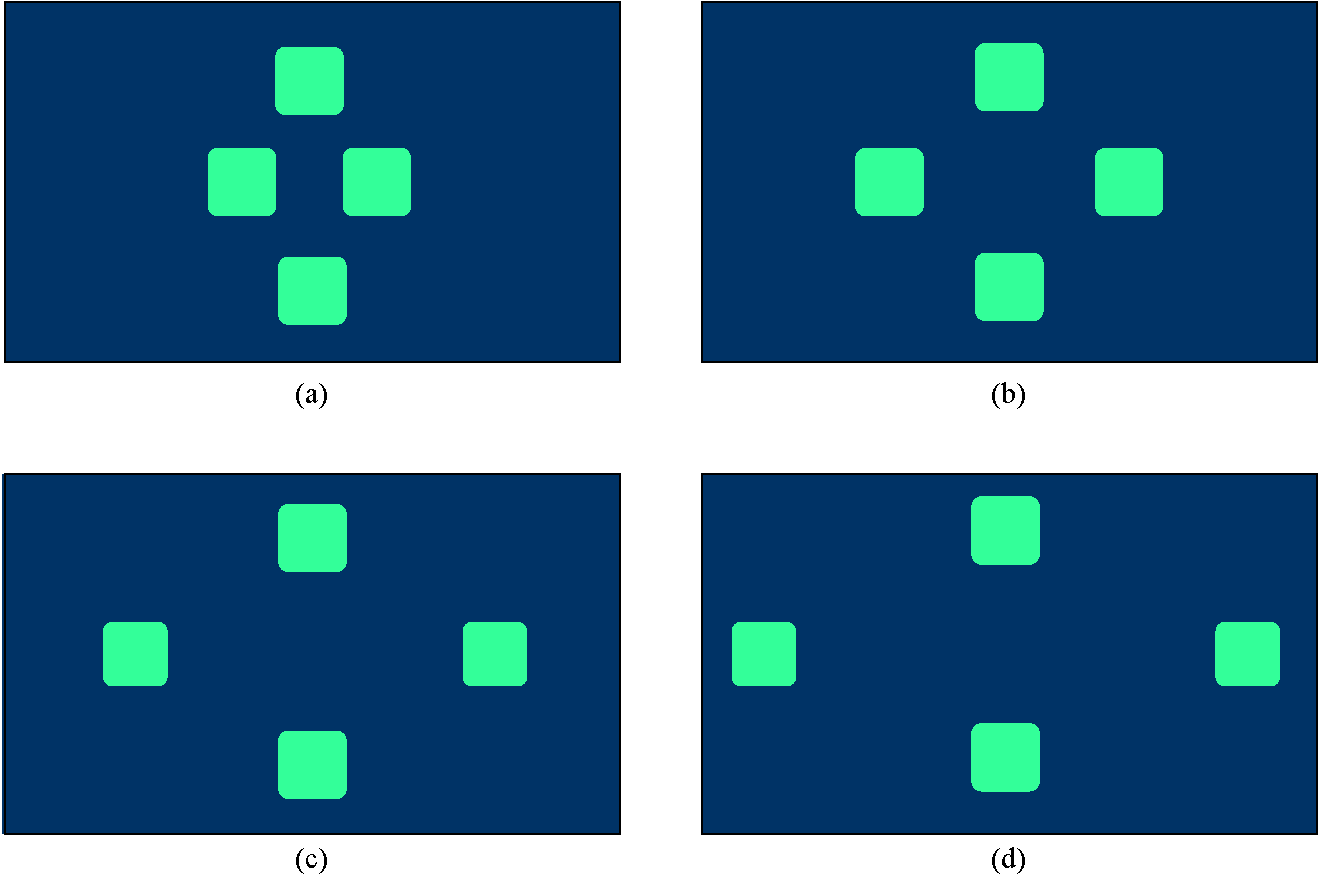
\includegraphics[width=0.75\textwidth]{grid-arrangements}
    \caption[Experimental SSVEP stimulus grid configurations adapted from \cite{zhao-stimulus-layout-effect}]{Experimental SSVEP stimulus grid configurations adapted from \cite{zhao-stimulus-layout-effect}. The absolute dimensions and positions of the stimulus squares and the background are not important here; only their relative positioning is relevant}
    \label{fig:ssvep-grid-arrangements}
\end{figure}

% \subsubsection{Filtering and signal preprocessing}
% Mention typical filtering choices - e.g. bandpass + 50Hz notch

% Decoding algos section
\section{Computational Approaches for SSVEP Decoding}
\subsection{Power spectral density and frequency domain}
Arguably the most obvious approach for analysing periodic signals in order to distinguish frequency content is through the use of Fourier analysis. Power spectral density analysis (PSDA) is typically used to analyse the power of a signal over a continuous frequency range. For a discrete time deterministic signal ${x[n]}$ with finite energy $\sum_{n=-\infty}^\infty |x[n]|^2 < \infty$, the discrete time Fourier transform (DTFT) is defined as 
\begin{equation}
    X(\omega)=\sum_{n=-\infty}^{\infty} x[n] e^{-j \omega n}
\end{equation}
The energy spectral density $S_x(\omega)$ of $x[n]$ is defined as $S_x(\omega) = |X(\omega)^2|$. The power spectral density (PSD) $P_x(\omega)$ of $x[n]$ of finite length $N$ is defined as 
\begin{equation}
P_x(\omega)=\lim _{N \rightarrow \infty} E\left\{\frac{1}{N}\left|\sum_{n=0}^{N-1} x[n] e^{-jn \omega}\right|^{2}\right\}
\end{equation}
The PSD represents the distribution of signal power over a frequency range of interest. In practice, one can only consider finite length signals with $N < \infty$ and so, $P_x(\omega)$ must be estimated (albeit arbitrarily closely). Such an estimate of power spectral density is called a \textbf{periodogram}.

In the context of SSVEP decoding, it is clear how PSDA could be useful. Simply by computing the periodogram (estimated PSD) of a measured EEG signal $x[n]$, the target SSVEP stimulus frequency $f^* \in \mathcal{F}$ could be inferred from the set of candidate stimulus frequencies $\mathcal{F}$ by choosing $f^* = \argmax_{f \in \mathcal{F}} P_x(\omega)$ where $\omega=2\pi f$. 

\subsubsection{Welch's method for PSD estimation}
Welch's method is commonly used to reduce noise in PSD analysis. This approach involves dividing the original signal into short overlapping windows of length $N^* \leq N$ which are then windowed (in the time domain). The periodograms of these windows are computed independently and then averaged. While this approach reduces variance in the final periodogram, it comes at the cost of decreased frequency resolution. Furthermore, the type of window used should be chosen carefully as this will further impact the resolution-variance trade off. Hamming, Blackman and Bartlett windows are popular choices.

\subsubsection{Efficacy of PSDA for SSVEP decoding}
\label{subsection:psda-vs-cca}
Many studies have demonstrated that PSDA can be used for SSVEP decoding/classification \cite{zhao-stimulus-layout-effect}, \cite{bci-survey-nicolas-alonso}, \cite{acampora-dataset}. However, it is widely documented that PSDA is inferior to more specialised statistical techniques that have been developed for this task: both in terms of signal classification accuracy and information transfer rate (ITR) \cite{autthasan-single-chan-ssvep}, \cite{lin-cca-2006}, \cite{sun-gcca}, \cite{zhang-mset-cca}, \cite{hakvoort-cca-psda-comparison}. The authors in \cite{hakvoort-cca-psda-comparison} performed a study specifically to compare the efficacy of PSDA vs statistical algorithms such as CCA (explored below) in EEG signal decoding. Their findings reinforce those of their colleagues in that CCA and its derivatives produce better decoding performance than PSDA.

\subsection{Statistical}

\subsubsection{Canonical correlation analysis (CCA)}
\label{subsection:CCA-c2}
CCA is a standard multivariate statistical technique for analysing multiple variables measured on a set of observations. In particular, variables are partitioned into two sets or \textit{views} of the data \cite{cca-tutorial}. Effectively, CCA is a multivariate extension of ordinary correlation. Given variable partitions $\mX \in \R^{m\times p}$, $\mY \in \R^{m\times q}$ each with $m$ observations, CCA seeks to find a linear combination of $\mX$, $\mY$ that maximises the correlation between their images $\vz_X = \mX\vw_X$ and $\vz_Y = \mY\vw_Y$. These images are known as the \textit{canonical variables} and $\vw_X$ and $\vw_Y$ are the \textit{canonical weight vectors} that effectively act as spatial filters across signal channels.

With CCA for SSVEP frequency recognition tasks, $\mX \in \R^{N_s\times N_c}$ is the set of \textit{measured} EEG signals from $N_c$ channels over $N_s$ observations. The measured signals in $\mX$ must be compared with each frequency $f_k \in \mathcal{F}$, a finite set of candidate stimulus frequencies. CCA can be used to compute weighted correlations between the measured signals and each candidate frequency $f_k$ by constructing a sinusoidal reference signal set $\mY_k \in \R^{N_s \times 2N_h}$ as follows: 

\begin{equation}
\mY_{k}=\left(\begin{array}{c}
\sin \left(2 \pi f_{k} t\right) \\
\cos \left(2 \pi f_{k} t\right) \\
\sin \left(4 \pi f_{k} t\right) \\
\cos \left(4 \pi f_{k} t\right) \\
\vdots \\
\sin \left(2 \pi N_h f_{k} t\right) \\
\cos \left(2 \pi N_h f_{k} t\right)
\end{array}\right), \quad t=\frac{1}{f_s}, \frac{2}{f_s}, \ldots, \frac{N_s}{f_s}
\label{eq:sinusoidal-ref}
\end{equation}

where $f_s$ is the sampling frequency and $N_h$ is the number of harmonics in the reference set, a parameter to be chosen. The scalp and other interacting layers between the brain and surface electrodes are both resistive and capacitive, producing low-pass filter dynamics \cite{baillet-em-brain-mapping}, \cite{lin-cca-2006}. Therefore, it is rare that more than $N_h=5$ harmonics are selected in the reference signal set \cite{lin-cca-2006}. The final task of frequency recognition is performed by selecting the frequency $f^*$
\begin{equation}
    f^* = \argmax_{f_k \in \mathcal{F}} \; \rho_k
    \label{eq:cca-freq-discrimination}
\end{equation}

corresponding to the candidate frequency $f_k$ which maximises the canonical correlation $\rho_k$ between $\mX$ and the the reference set $\mY_k$. While standard CCA is a good starting point for statistical SSVEP decoding as it forms the basis of many similar algorithms, there are several extensions which have been shown to significantly improve signal recognition performance \cite{zhang-mset-cca}, \cite{sun-gcca}, \cite{miao-hybrid-cca}. The most promising of these are explored below.

\subsubsection{Task-related component analysis (TRCA)}
\label{section:trca-c2}
Task-related component analysis (TRCA) as a decoding technique in biophysical systems was introduced in the seminal paper by Tanaka \textit{et al} \cite{tanaka-trca}. TRCA seeks to extract task-related signal components (as opposed to spurious, unwanted components such as EMG artefacts and background noise) by identifying components that lead to maximum reproducibility across trials. Task-related components are constructed as linear combinations of signals recorded across multiple time blocks (trials) and their weights are optimised so as to maximise their inter-block correlation or covariance \cite{tanaka-trca}. Components with maximum inter-block covariance and thus, reproducibility or consistency, are identified as task-related components (subject to certain significance measures as discussed later). Further advantages of TRCA are that, unlike other more common generalised linear models (GLMs), it assumes no \textit{a priori} knowledge of source signals and is not sensitive to autocorrelation \cite{tanaka-trca}. It also offers concrete measures of task-relatedness unlike some other data-driven methods like independent component analysis.

To illustrate the basic idea of this algorithm, \cite{tanaka-trca} presents a useful toy example. Consider a task-related signal $s(t)$ standardised to have zero mean and unit variance embedded in additive white (uncorrelated) noise $n(t)$: $x(t) = a_1s(t) + a_2n(t)$ with some mixing scalars $a_i \in \R$. Then, assume the observable signal $x(t)$ is measured over two distinct time blocks or trials to yield $x_1(t)$ and $x_2(t)$. A linear model of the two observed blocks could be defined as follows:
\begin{align}
    x_1(t) = a_{11}s(t) + a_{12}n(t) \\
    x_2(t) = a_{21}s(t) + a_{22}n(t)
\end{align}
As mentioned above, TRCA attempts to recover task related components (only $s(t)$ in this case) from a linear combination of observations across trials. Defining this weighted sum as $y(t)$ with 
\begin{equation}
    y(t)= y_1(t) + y_2(t) = w_{1} x_{1}(t)+w_{2} x_{2}(t)=\left(w_{1} a_{11}+w_{2} a_{21}\right) s(t)+\left(w_{1} a_{12}+w_{2} a_{22}\right) n(t)
\end{equation}
Recovering $s(t)$ involves maximising the covariance between $y_1(t)$ and $y_2(t)$:
\begin{align}
\begin{split}
\operatorname{Cov}\left(y_1, y_2\right)=&\left(w_{1} a_{11}+w_{2} a_{21}\right)^{2} \operatorname{Cov}\left(s_1, s_2\right)
+\left(w_{1} a_{12}+w_{2} a_{22}\right)^{2} \operatorname{Cov}\left(n_{1}, n_2\right) \\
&+\left(w_{1} a_{11}+w_{2} a_{21}\right)\left(w_{1} a_{12}+w_{2} a_{22}\right)\left[\operatorname{Cov}\left(s_{2}, n_2\right)\right
\left.+\operatorname{Cov}\left(n_{1}, s_2\right)\right]
\end{split}
\\
\notag
=&\left(w_{1} a_{11}+w_{2} a_{21}\right)^{2} \operatorname{Cov}\left(s_{1}, s_2\right)
\end{align}
Since $\operatorname{Cov}(n_1, n_2) = \operatorname{Cov}(s_1, n_2) = \operatorname{Cov}(n_1, s_2) = 0$. In order to bound this quadratic objective, we choose the weights $w_1, w_2$ so that the variance of $y$ is constrained to 1:
\begin{equation}
    \operatorname{var}(y)=\left(w_{1} a_{11}+w_{2} a_{21}\right)^{2}+\left(w_{1} a_{12}+w_{2} a_{22}\right)^{2}=1
\end{equation}
where $s(t)$ and $n(t)$ are also assumed to be uncorrelated $\forall t$. The solution of this constrained optimisation problem is 
\begin{equation}
    w_{1} a_{11}+w_{2} a_{21} = 1, \quad w_{1} a_{12}+w_{2} a_{22} = 0, 
\end{equation}
which, barring the unlikely case that $a_{11}a_{22} = a_{12}a_{21}$, yields $y(t)=s(t)$ as desired. This demonstrates how inter-trial covariance maximisation can be used for recovery of task-related signals.

Although TRCA has been shown to outperform CCA \cite{lee-trca-2step}, \cite{miao-hybrid-cca}, \cite{sun-gcca}, extended and hybrid forms of these algorithms have produced superior results. Some of these extensions are explored below.

\subsubsection{Multiset canonical correlation analysis (MsetCCA)}
\label{subsection:mset-cca-c2}
MsetCCA is one extension of standard CCA that takes into account historical data instead of performing inference purely on new observations. Zhang \textit{et al} propose that this is one of the reasons that standard CCA performs poorly on short time windows; it effectively over fits to localised dynamics \cite{zhang-mset-cca}. Furthermore, the authors suggest that exclusively using the pre-constructed sinusoidal reference set is not optimal since this artificial reference does not include other features from real EEG data \cite{zhang-mset-cca}. To circumvent this, MsetCCA seeks to optimise the reference signals used in the CCA algorithm by learning multiple linear transforms to maximise overall correlation between canonical variables over \textit{many} sets of EEG data at each candidate frequency $f_k \in \mathcal{F}$ \cite{zhang-mset-cca}. This optimisation effectively finds optimal joint spatial filters $\vw_1, \dots, \vw_{N_t}$ (over $N_t$ trials) using only historical observations (`training' data). The authors claim that MsetCCA outperforms similar techniques, especially in cases with few channels and short time windows. 

\subsubsection{Generalised canonical correlation analysis (GCCA)}
\label{subsection:gcca-c2}
Wong \textit{et al} noted in their study of EEG spatial filtering methods in \cite{wong-spatial-filt} that only using historical observations to estimate spatial filters (canonical weights) $\vw_i$, as in MsetCCA, is not optimal. Using both historical data and pre-constructed sinusoidal reference signals as with standard CCA was found to enhance the algorithm's robustness and reduced calibration requirements \cite{wong-spatial-filt}.  Motivated by this, the authors in \cite{sun-gcca} developed a new algorithm called generalised CCA (GCCA) that aims to simultaneously maximise correlation between three sets of data: historical observations, measured signals in a new sample and the pre-constructed sinusoidal reference. As interpreted by the authors in \cite{sun-gcca}, the optimal spatial filters obtained through GCCA perform SSVEP signal denoising.

\subsection{Data-driven and machine learning}

\section{Existing BCI Technology}
\label{section:existing-bci-tech-c2}
Commercial BCI devices are currently available from several manufacturers, including but not limited to: B-Alert X10, NeuroSky, Emotiv and OpenBCI. These devices are typically targeted at consumers but some are also aimed at research applications (such as the Emotiv Epoc Flex). This review will not explore these devices further as they are all priced in excess of several hundred USD which violates the important budget constrain on this project.

More of interest to this project is the low-cost, lightweight BCI devices being developed in the EEG research community. Several studies have presented promising BCI prototypes that have demonstrated that reliable EEG signal decoding is possible in significantly resource-constrained settings \cite{uktveris-modular-bci}, \cite{de-vos-p300-speller}, \cite{liao-gaming-control}, \cite{chai-embedded-bci}, \cite{acampora-svm-clf}. In particular, these studies have explored devices that are constrained in terms of computing capacity, mobility or form factor, number of channels available and cost. 

However, a thorough review of these existing BCI prototypes did not reveal any that satisfied all constraints or requirements of this project. Uktveris \textit{et al} demonstrated a very promising and impressive device with wireless capabilities (communication with a host PC or other device using BLE and/or Wi-Fi) and some on-device digital signal processing ability \cite{uktveris-modular-bci}. However, their device requires final signal decoding to be performed on a host device separate from the actual BCI itself. Furthermore, the cost of the raw materials in their project was around 113 EUR \cite{uktveris-modular-bci} (albeit for a more capable multi-channel BCI system).

The authors in \cite{chai-embedded-bci} created an embedded BCI system consisting of a small, on-board analogue sampling device that communicates using RF signals with another external main controller. The authors claim this to be a `wireless' BCI but in fact, all computation and decoding happens on the fixed main controller and the on-board controller only serves to acquire the raw signals. 

Acampora \textit{et al} provide a slightly more feasible prototype in \cite{acampora-dataset} and provide an expansion for SSVEP decoding using this device in \cite{acampora-svm-clf}. This device was able to achieve maximum SSVEP classification accuracy of $74.5\%$ for a 2s recording window, and up to $92.7\%$ over a 4s window (using a support vector machine with Gaussian or RBF kernel) \cite{acampora-svm-clf}. However, this prototype utilises an off-the-shell Olimex EEG-SMT device for signal acquisition and a Raspberry Pi 3 for computation and decoding. While their device is seemingly effective and fairly mobile, it would certainly not satisfy the £20 price budget in this project. Housing a Raspberry Pi 3 and battery pack along with the rest of the BCI hardware would also be overly cumbersome for this project.